\documentclass[11pt,]{article}
\usepackage{lmodern}
\usepackage{amssymb,amsmath}
\usepackage{ifxetex,ifluatex}
\usepackage{fixltx2e} % provides \textsubscript
\ifnum 0\ifxetex 1\fi\ifluatex 1\fi=0 % if pdftex
  \usepackage[T1]{fontenc}
  \usepackage[utf8]{inputenc}
\else % if luatex or xelatex
  \ifxetex
    \usepackage{mathspec}
  \else
    \usepackage{fontspec}
  \fi
  \defaultfontfeatures{Ligatures=TeX,Scale=MatchLowercase}
\fi
% use upquote if available, for straight quotes in verbatim environments
\IfFileExists{upquote.sty}{\usepackage{upquote}}{}
% use microtype if available
\IfFileExists{microtype.sty}{%
\usepackage{microtype}
\UseMicrotypeSet[protrusion]{basicmath} % disable protrusion for tt fonts
}{}
\usepackage[margin = 1.5in]{geometry}
\usepackage{hyperref}
\PassOptionsToPackage{usenames,dvipsnames}{color} % color is loaded by hyperref
\hypersetup{unicode=true,
            pdftitle={Financial Time Series},
            pdfauthor={Abhinav Anand, IIMB},
            colorlinks=true,
            linkcolor=blue,
            citecolor=magenta,
            urlcolor=red,
            breaklinks=true}
\urlstyle{same}  % don't use monospace font for urls
\usepackage{color}
\usepackage{fancyvrb}
\newcommand{\VerbBar}{|}
\newcommand{\VERB}{\Verb[commandchars=\\\{\}]}
\DefineVerbatimEnvironment{Highlighting}{Verbatim}{commandchars=\\\{\}}
% Add ',fontsize=\small' for more characters per line
\usepackage{framed}
\definecolor{shadecolor}{RGB}{248,248,248}
\newenvironment{Shaded}{\begin{snugshade}}{\end{snugshade}}
\newcommand{\KeywordTok}[1]{\textcolor[rgb]{0.13,0.29,0.53}{\textbf{#1}}}
\newcommand{\DataTypeTok}[1]{\textcolor[rgb]{0.13,0.29,0.53}{#1}}
\newcommand{\DecValTok}[1]{\textcolor[rgb]{0.00,0.00,0.81}{#1}}
\newcommand{\BaseNTok}[1]{\textcolor[rgb]{0.00,0.00,0.81}{#1}}
\newcommand{\FloatTok}[1]{\textcolor[rgb]{0.00,0.00,0.81}{#1}}
\newcommand{\ConstantTok}[1]{\textcolor[rgb]{0.00,0.00,0.00}{#1}}
\newcommand{\CharTok}[1]{\textcolor[rgb]{0.31,0.60,0.02}{#1}}
\newcommand{\SpecialCharTok}[1]{\textcolor[rgb]{0.00,0.00,0.00}{#1}}
\newcommand{\StringTok}[1]{\textcolor[rgb]{0.31,0.60,0.02}{#1}}
\newcommand{\VerbatimStringTok}[1]{\textcolor[rgb]{0.31,0.60,0.02}{#1}}
\newcommand{\SpecialStringTok}[1]{\textcolor[rgb]{0.31,0.60,0.02}{#1}}
\newcommand{\ImportTok}[1]{#1}
\newcommand{\CommentTok}[1]{\textcolor[rgb]{0.56,0.35,0.01}{\textit{#1}}}
\newcommand{\DocumentationTok}[1]{\textcolor[rgb]{0.56,0.35,0.01}{\textbf{\textit{#1}}}}
\newcommand{\AnnotationTok}[1]{\textcolor[rgb]{0.56,0.35,0.01}{\textbf{\textit{#1}}}}
\newcommand{\CommentVarTok}[1]{\textcolor[rgb]{0.56,0.35,0.01}{\textbf{\textit{#1}}}}
\newcommand{\OtherTok}[1]{\textcolor[rgb]{0.56,0.35,0.01}{#1}}
\newcommand{\FunctionTok}[1]{\textcolor[rgb]{0.00,0.00,0.00}{#1}}
\newcommand{\VariableTok}[1]{\textcolor[rgb]{0.00,0.00,0.00}{#1}}
\newcommand{\ControlFlowTok}[1]{\textcolor[rgb]{0.13,0.29,0.53}{\textbf{#1}}}
\newcommand{\OperatorTok}[1]{\textcolor[rgb]{0.81,0.36,0.00}{\textbf{#1}}}
\newcommand{\BuiltInTok}[1]{#1}
\newcommand{\ExtensionTok}[1]{#1}
\newcommand{\PreprocessorTok}[1]{\textcolor[rgb]{0.56,0.35,0.01}{\textit{#1}}}
\newcommand{\AttributeTok}[1]{\textcolor[rgb]{0.77,0.63,0.00}{#1}}
\newcommand{\RegionMarkerTok}[1]{#1}
\newcommand{\InformationTok}[1]{\textcolor[rgb]{0.56,0.35,0.01}{\textbf{\textit{#1}}}}
\newcommand{\WarningTok}[1]{\textcolor[rgb]{0.56,0.35,0.01}{\textbf{\textit{#1}}}}
\newcommand{\AlertTok}[1]{\textcolor[rgb]{0.94,0.16,0.16}{#1}}
\newcommand{\ErrorTok}[1]{\textcolor[rgb]{0.64,0.00,0.00}{\textbf{#1}}}
\newcommand{\NormalTok}[1]{#1}
\usepackage{graphicx,grffile}
\makeatletter
\def\maxwidth{\ifdim\Gin@nat@width>\linewidth\linewidth\else\Gin@nat@width\fi}
\def\maxheight{\ifdim\Gin@nat@height>\textheight\textheight\else\Gin@nat@height\fi}
\makeatother
% Scale images if necessary, so that they will not overflow the page
% margins by default, and it is still possible to overwrite the defaults
% using explicit options in \includegraphics[width, height, ...]{}
\setkeys{Gin}{width=\maxwidth,height=\maxheight,keepaspectratio}
\IfFileExists{parskip.sty}{%
\usepackage{parskip}
}{% else
\setlength{\parindent}{0pt}
\setlength{\parskip}{6pt plus 2pt minus 1pt}
}
\setlength{\emergencystretch}{3em}  % prevent overfull lines
\providecommand{\tightlist}{%
  \setlength{\itemsep}{0pt}\setlength{\parskip}{0pt}}
\setcounter{secnumdepth}{0}
% Redefines (sub)paragraphs to behave more like sections
\ifx\paragraph\undefined\else
\let\oldparagraph\paragraph
\renewcommand{\paragraph}[1]{\oldparagraph{#1}\mbox{}}
\fi
\ifx\subparagraph\undefined\else
\let\oldsubparagraph\subparagraph
\renewcommand{\subparagraph}[1]{\oldsubparagraph{#1}\mbox{}}
\fi

%%% Use protect on footnotes to avoid problems with footnotes in titles
\let\rmarkdownfootnote\footnote%
\def\footnote{\protect\rmarkdownfootnote}

%%% Change title format to be more compact
\usepackage{titling}

% Create subtitle command for use in maketitle
\newcommand{\subtitle}[1]{
  \posttitle{
    \begin{center}\large#1\end{center}
    }
}

\setlength{\droptitle}{-2em}

  \title{Financial Time Series}
    \pretitle{\vspace{\droptitle}\centering\huge}
  \posttitle{\par}
    \author{Abhinav Anand, IIMB}
    \preauthor{\centering\large\emph}
  \postauthor{\par}
      \predate{\centering\large\emph}
  \postdate{\par}
    \date{2018/07/16}

\linespread{1.25}
\usepackage{amsmath}

\begin{document}
\maketitle

\section{Background}\label{background}

Financial prices, indices, returns etc. are sequences of real numbers
indexed by time. The study of their mathematical and statistical
properties is vital for those aspiring to write papers in empirical
finance.

As an illustration we produce the daily time series for the closing
value of the Bombay Stock Exchange index (``Sensex'').

\begin{Shaded}
\begin{Highlighting}[]
\NormalTok{file_bse <-}\StringTok{ "SENSEX.csv"}
\NormalTok{index_bse <-}\StringTok{ }\NormalTok{readr}\OperatorTok{::}\KeywordTok{read_csv}\NormalTok{(file_bse)}
\NormalTok{index_bse}\OperatorTok{$}\NormalTok{Date <-}\StringTok{ }\KeywordTok{as.Date}\NormalTok{(index_bse}\OperatorTok{$}\NormalTok{Date, }\DataTypeTok{format =} \StringTok{"%d-%B-%Y"}\NormalTok{)}

\KeywordTok{plot}\NormalTok{(index_bse}\OperatorTok{$}\NormalTok{Date,}
\NormalTok{     index_bse}\OperatorTok{$}\NormalTok{Close,}
     \DataTypeTok{type =} \StringTok{"l"}\NormalTok{,}
     \DataTypeTok{col =} \StringTok{"blue"}\NormalTok{,}
     \DataTypeTok{xlab =} \StringTok{"Year"}\NormalTok{,}
     \DataTypeTok{ylab =} \StringTok{"BSE Index"}\NormalTok{,}
     \DataTypeTok{main =} \StringTok{"Indian stock market performance"}
\NormalTok{     )}
\NormalTok{fit_lm <-}\StringTok{ }\KeywordTok{lm}\NormalTok{(Close }\OperatorTok{~}\StringTok{ }\NormalTok{Date, }
             \DataTypeTok{data =}\NormalTok{ index_bse) }\CommentTok{#fit linear model}
\KeywordTok{abline}\NormalTok{(fit_lm, }\CommentTok{#plot linear model line}
       \DataTypeTok{lty =} \StringTok{"dotdash"}\NormalTok{, }
       \DataTypeTok{col =} \StringTok{"red"}\NormalTok{,}
       \DataTypeTok{lwd =} \DecValTok{2}
\NormalTok{       )}
\end{Highlighting}
\end{Shaded}

\begin{center}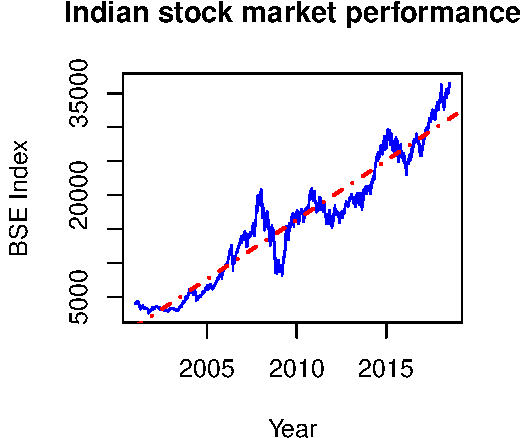
\includegraphics{FMC_T4_PhD_Fin_Time_Series_files/figure-latex/BSE-1} \end{center}

\begin{Shaded}
\begin{Highlighting}[]
\CommentTok{# via ggplot}

\KeywordTok{ggplot}\NormalTok{(}\DataTypeTok{data =}\NormalTok{ index_bse, }
       \KeywordTok{aes}\NormalTok{(Date, Close)}
\NormalTok{       ) }\OperatorTok{+}
\StringTok{  }\KeywordTok{geom_line}\NormalTok{(}\DataTypeTok{lwd =} \FloatTok{0.3}\NormalTok{,}
            \DataTypeTok{color =} \StringTok{"blue"}
\NormalTok{            ) }\OperatorTok{+}
\StringTok{  }\KeywordTok{geom_smooth}\NormalTok{(}\DataTypeTok{method =} \StringTok{"lm"}\NormalTok{,}
              \DataTypeTok{lty =} \StringTok{"dotdash"}\NormalTok{,}
              \DataTypeTok{lwd =} \FloatTok{0.6}\NormalTok{,}
              \DataTypeTok{color =} \StringTok{"red"}\NormalTok{,}
              \DataTypeTok{se =}\NormalTok{ F) }\OperatorTok{+}
\StringTok{  }\KeywordTok{theme_minimal}\NormalTok{() }\OperatorTok{+}
\StringTok{  }\KeywordTok{labs}\NormalTok{(}\DataTypeTok{x =} \StringTok{"Years"}\NormalTok{,}
       \DataTypeTok{y =} \StringTok{"BSE Sensex"}\NormalTok{,}
       \DataTypeTok{title =} \StringTok{"Indian stock market performance"}
\NormalTok{       )}
\end{Highlighting}
\end{Shaded}

\begin{center}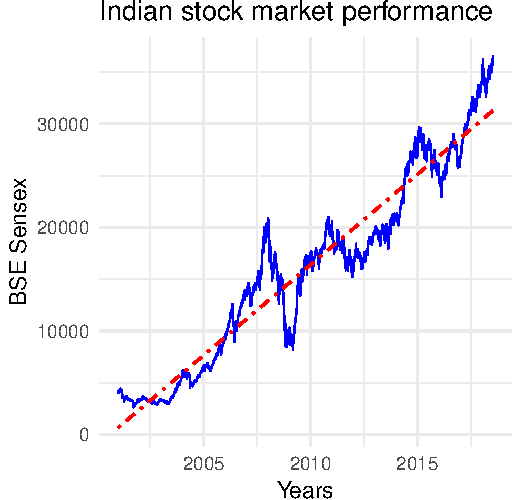
\includegraphics{FMC_T4_PhD_Fin_Time_Series_files/figure-latex/BSE-2} \end{center}

It seems that the level of the series is rising and the fluctuations are
sometimes high and sometimes low.

This index series is an example of a \emph{non-stationary} time series.
This roughly means that the mean and the variance of such a series are
functions of time.

Here is another example of an index series that seems non-stationary:
the cumulative price index (CPI) for India where the level in 2010 is
standardized to 100.

\begin{Shaded}
\begin{Highlighting}[]
\NormalTok{file_cpi <-}\StringTok{ "IND_CPI_ALL_2010_100.csv"}
\NormalTok{ind_cpi <-}\StringTok{ }\NormalTok{readr}\OperatorTok{::}\KeywordTok{read_csv}\NormalTok{(file_cpi)}

\NormalTok{ind_cpi <-}\StringTok{ }\NormalTok{ind_cpi }\OperatorTok
\StringTok{  }\NormalTok{dplyr}\OperatorTok{::}\KeywordTok{rename}\NormalTok{(}\StringTok{"CPI"}\NormalTok{ =}\StringTok{ }\NormalTok{INDCPIALLMINMEI)}

\KeywordTok{ggplot}\NormalTok{(ind_cpi, }
       \KeywordTok{aes}\NormalTok{(DATE, CPI)}
\NormalTok{       ) }\OperatorTok{+}
\StringTok{  }\KeywordTok{geom_line}\NormalTok{(}\DataTypeTok{color =} \StringTok{"blue"}\NormalTok{) }\OperatorTok{+}
\StringTok{  }\KeywordTok{geom_smooth}\NormalTok{(}\DataTypeTok{method =} \StringTok{"lm"}\NormalTok{,}
              \DataTypeTok{lty =} \StringTok{"dotdash"}\NormalTok{,}
              \DataTypeTok{lwd =} \FloatTok{0.6}\NormalTok{,}
              \DataTypeTok{se =}\NormalTok{ F,}
              \DataTypeTok{color =} \StringTok{"red"}
\NormalTok{              ) }\OperatorTok{+}
\StringTok{  }\KeywordTok{theme_minimal}\NormalTok{() }\OperatorTok{+}
\StringTok{  }\KeywordTok{labs}\NormalTok{(}\DataTypeTok{x =} \StringTok{"Years"}\NormalTok{,}
       \DataTypeTok{y =} \StringTok{"CPI: India"}
\NormalTok{       )}
\end{Highlighting}
\end{Shaded}

\begin{center}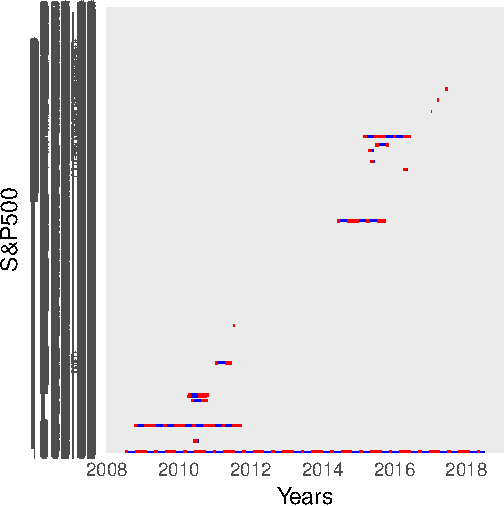
\includegraphics{FMC_T4_PhD_Fin_Time_Series_files/figure-latex/CPI_Ind-1} \end{center}

\section{Returns}\label{returns}

We observe prices in the financial markets empirically. However, due to
their non-stationary nature, they are hard to analyze. Hence they are
converted to return series which are usually stationary. There are many
ways to construct different notions of returns from the same underlying
price sequence. We discuss some prominent ones below.

\subsection{One-Period Simple Return}\label{one-period-simple-return}

The simple one period return for holding some asset whose price is given
by the sequence \(\{p_t\}_{t=1}^n\) is:

\[r_t := \frac{p_t-p_{t-1}}{p_{t-1}} = \frac{p_t}{p_{t-1}}-1\]

\subsection{Multi-period Simple
Return}\label{multi-period-simple-return}

\[r_t[k] := \frac{p_t-p_{t-k}}{p_{t-k}} = \frac{p_t}{p_{t-k}}-1\]
\[r_t[k] := \frac{p_t}{p_{t-k}}-1 = 
\frac{p_t}{p_{t-1}}\hdots\frac{p_{t-k+1}}{p_t-k}-1\]
\[r_t[k] := (1+r_t)\hdots(1+r_{t-k+1})-1\]

\section*{References}\label{references}
\addcontentsline{toc}{section}{References}

\hypertarget{refs}{}
\hypertarget{ref-Jondeau_Poon_Rockinger:2007}{}
Jondeau, Eric, Ser-Huang Poon, and Michael Rockinger. 2007.
\emph{Financial Modeling Under Non-Gaussian Distributions}. Springer
Finance.

\hypertarget{ref-Tsay:2010}{}
Tsay, Ruey S. 2010. \emph{Analysis of Financial Time Series}. Third
Edition. John Wiley; Sons.


\end{document}
